\documentclass[11pt,a4paper]{article}

\usepackage[margin=1in]{geometry}
\usepackage{graphicx}
\usepackage{booktabs}
\usepackage{amsmath,amssymb}
\usepackage{hyperref}
\usepackage{listings}
\usepackage{xcolor}
\usepackage{float}
\usepackage{natbib}

\graphicspath{{figures/}}

\title{\textbf{Precision Flow Conditioning for Hydrodynamic Cavitation Experiments}\\[0.4em]
\large HDD Platter Tesla-Style Disc Stack with Optional Central HVAT}
\author{George Lambert \\ Litchfield, NH \\ \href{mailto:marchon@gmail.com}{marchon@gmail.com} \\ \href{https://www.linkedin.com/in/podjacker}{linkedin.com/in/podjacker}}
\date{\today}

\begin{document}

\maketitle

\begin{abstract}
A fully parametric, low-cost, 3D-printable flow conditioner built from 25 polished Enterprise 3.5" HDD platters is presented. The device uses a stationary (or lightly braked) Tesla-style boundary-layer spiral to deliver highly uniform, low-turbulence gas or liquid injection into a cavitation chamber. An optional central Hybrid Vertical Axis Turbine (HVAT) rotor further organizes the exit flow. The design is optimized for repeatability in Greenyer/MFMP-style cavitation and LENR experiments (hydrodynamic + ultrasonic hybrids, bubble dynamics, foil erosion, gas evolution, and anomalous effects studies). Complete OpenSCAD sources, BOM, assembly instructions, and testing protocols are provided.

\textbf{Important Limitation:} All performance estimates, graphs, and "what-if" scenarios in this document are based on simplified analytical models. They are conceptual tools only and have not been validated by CFD or physical experiments by the author. See the project documentation for a full statement of current limitations.
\end{abstract}

\section{Introduction}

Standard Tesla turbines are boundary-layer devices that convert fluid kinetic energy into shaft torque via viscous drag on closely spaced smooth discs \cite{tesla1913,rice1965}. The flow enters tangentially at the periphery and spirals inward to a central exhaust.

In this work the same geometry is deliberately repurposed: the disc stack is run essentially stationary and its function is inverted — it becomes a precision \emph{flow conditioner} whose output is a clean, repeatable, multi-channel spiral jet ideally suited for controlled cavitation bubble generation.

The motivation comes directly from open LENR/cavitation research (Bob Greenyer and the Martin Fleischmann Memorial Project) \cite{greenyer2020,greenyer2026,greenyer2023}. Many of the most interesting effects (microsphere formation, anomalous elemental changes, ``strange radiation'', excess heat signatures) appear to depend sensitively on bubble size distribution, collapse intensity, and the presence of dissolved or injected gases (including deuterium) \cite{brennen1995,franc2004}. Crude injection methods introduce large run-to-run variability. A device that can deliver well-characterized, low-turbulence, tunable flow therefore has immediate scientific value.

\section{Device Architecture}

\subsection{Platter Stack}
\begin{itemize}
    \item 25 Enterprise 3.5'' HDD platters (95 mm OD, $\approx 0.9$ mm thick, mirror-polished)
    \item Nominal 1.0 mm inter-platter gaps (24 printed spacer rings)
    \item Active stack height $\approx 47$ mm
\end{itemize}

The highly polished surfaces and tight, uniform gaps create many parallel, low-Reynolds-number channels. Fluid entering from the tangential nozzles develops a strong inward spiral while remaining attached to the disc surfaces via the boundary-layer effect.

\subsection{Tangential Nozzles}
Six nozzles equally spaced around the periphery, oriented 8--12° from true tangential (10° default). This angle was found through iteration to give a vigorous yet stable spiral without excessive radial velocity or flow separation at the entry.

\subsection{Central HVAT (Hybrid Vertical Axis Turbine)}
A small (28 mm diameter) hybrid rotor combining Savonius starting scoops with helical Darrius blades (a configuration inspired by classic VAWT research \cite{savonius1925,darrieus1931,akwa2012,paraschivoiu2002,liang2017}) is mounted on bearings in the central exhaust region. It is \emph{not} optimized for net power extraction. Instead it uses residual swirl energy to further straighten and organize the flow into a cleaner axial jet before the final diffuser and cavitation nozzle. The rotor can be left free, lightly braked (printed caliper), or driven.

\subsection{Cavitation Nozzle}
A Venturi-style converging-diverging nozzle with interchangeable orifice inserts (6/8/10/12 mm throat) accelerates the conditioned flow and creates the sharp pressure drop required for reproducible bubble inception immediately upstream of (or inside) the experimental chamber.

\section{Key Equations}

\textbf{Reynolds number in the gaps} (characteristic length = gap height) \cite{brennen1995}:
\[
Re = \frac{\rho v g}{\mu}
\]
where $g$ is the inter-platter gap, $v$ the local velocity.

\textbf{Cavitation number} at the nozzle exit \cite{brennen1995,franc2004}:
\[
\sigma = \frac{p_\text{static} - p_\text{vapor}}{\frac{1}{2}\rho v^2}
\]
Typical inception for sharp orifices occurs for $\sigma \lesssim 2$--3 depending on geometry and dissolved gas content.

\textbf{Approximate spiral velocity scaling} (order-of-magnitude from continuity + boundary layer considerations):
\[
v_\theta(r) \approx v_\text{nozzle} \cdot \frac{r_\text{nozzle}}{r} \cdot f(\text{gap}, \text{Re})
\]

Full quantitative modeling requires CFD on the actual STL geometry.

\section{Open Source Deliverables}

All design artifacts are released under appropriate open licenses (CERN OHL-S-2 for hardware, MIT for software/docs). This work builds upon decades of open research and open-source tooling, including the original Tesla turbine concept \cite{tesla1913}, modern boundary-layer turbine analysis \cite{rice1965,sengupta2016}, and the experimental cavitation protocols developed by Bob Greenyer and the MFMP community \cite{greenyer2020,greenyer2026}.

The following tools were essential to this project:
\begin{itemize}
    \item OpenSCAD \cite{openscad2025} for all parametric 3D models.
    \item Python scientific stack (NumPy \cite{numpy2025}, Matplotlib \cite{matplotlib2025}, Pillow \cite{pillow2025}, SciPy \cite{scipy2025}) used to generate engineering drawings, performance graphs, flow animations, and DXF profiles \cite{flow_conditioner_generators2026}.
    \item \TeX{} Live 2026 \cite{texlive2026} and supporting tools such as Inkscape \cite{inkscape2025}.
\end{itemize}

\begin{itemize}
    \item Parametric OpenSCAD files (main housing, HVAT blades, spacers, jigs, sensor mounts, full cavitation nozzle with orifice family)
    \item Complete BOM (see \texttt{data/BOM.csv})
    \item Step-by-step assembly instructions and testing protocol for Greenyer-style experiments
    \item Python engineering models (Reynolds, cavitation number, rough velocity estimates)
    \item Custom Python generators for engineering drawings, DXF fabrication profiles, flow path animations, and performance sensitivity graphs \cite{flow_conditioner_generators2026}
    \item This document + accompanying Sphinx site
\end{itemize}

The entire package is intended to be immediately buildable by anyone with a consumer 3D printer and a stack of dead Enterprise hard drives.

\section{Tools and Software}

This project relies on a modern open-source toolchain for design, analysis, visualization, and documentation. The following tools were used extensively:

\begin{itemize}
    \item \textbf{OpenSCAD} \cite{openscad2025} — parametric CAD modeling of all components.
    \item \textbf{FreeCAD} \cite{freecad2025} — STL to STEP conversion and additional modeling.
    \item \textbf{Python 3} \cite{python2025} with NumPy \cite{numpy2025}, Matplotlib \cite{matplotlib2025}, Pillow \cite{pillow2025}, and SciPy \cite{scipy2025}.
    \item Custom generators developed for this project \cite{flow_conditioner_generators2026} (engineering drawings, DXF export, flow animation frames, and performance sensitivity plots).
    \item \TeX{} Live 2026 \cite{texlive2026} and Inkscape \cite{inkscape2025} for documentation and figure preparation.
\end{itemize}

These tools enabled the creation of the engineering drawings, cutaway views, animated flow visualizations, DXF fabrication profiles, and quantitative performance graphs presented throughout this work.

\section{Conclusion}

By inverting the usual purpose of a Tesla disc stack and adding a modest active straightener (the HVAT), we obtain a compact, low-cost, highly reproducible precision injection tool for cavitation physics. The design directly supports the open, low-budget, high-documentation experimental ethos of the MFMP community.

Future work includes full CFD validation, integrated instrumentation, deuterium-specific protocols, and systematic comparison against simpler injection methods using the same ultrasonic + foil diagnostics that have become standard in the field.

\section*{Acknowledgments}
This project was conceived and developed by George Lambert (Litchfield, NH) in collaboration with Grok (xAI) in May 2026. Significant portions of the technical implementation, documentation, diagrams, OpenSCAD modules, Python tooling, and LaTeX work were generated with assistance from SuperGrok Heavy (@grokbuild-beta).

The design draws heavy inspiration from the open research of Bob Greenyer and the Martin Fleischmann Memorial Project (MFMP) \cite{greenyer2020,greenyer2026}.

Contact: \href{mailto:marchon@gmail.com}{marchon@gmail.com} \quad | \quad \href{https://www.linkedin.com/in/podjacker}{linkedin.com/in/podjacker}

\section*{Limitations and Scope}
All performance estimates, graphs, bubble size models, and "what-if" scenarios presented in this document are derived from highly simplified analytical approximations. They are intended for educational exploration and hypothesis generation only.

This work does not contain:
- Computational Fluid Dynamics (CFD) validation
- Experimental data from physical builds by the author
- Validated performance predictions

Readers are strongly encouraged to treat all such material as conceptual. Real-world behavior will depend on manufacturing precision, surface finish, alignment, fluid properties, and many other factors. Independent experimental validation by builders is essential before any scientific conclusions can be drawn.

A more detailed statement of the current project status is available in the accompanying Sphinx documentation.

**Maturity Matrix (May 2026)**

\begin{tabular}{lll}
\textbf{Area} & \textbf{Maturity} & \textbf{Reliability} \\
Physical CAD \& BOM & Good & Reasonable for building \\
3D Printing Documentation & Good & Mostly reliable \\
Performance Graphs \& Models & Very Low & Do not rely on them \\
Experimental Validation (by author) & None & None exists \\
Proven as Consistent Testbed & Unknown & Unproven \\
\end{tabular}

The project is currently best understood as a well-documented open hardware starting point rather than a finished, validated scientific platform.

\section{Fabrication Package \& Engineering Drawings}

All components are designed for straightforward FDM 3D printing in PETG or ABS. The drawings below document the complete set of printable parts for the default 25-platter configuration.

\subsection{Main Housing and Nozzles}
The primary structural element contains six tangential inlets at approximately 10° from true tangent. Figure~\ref{fig:housing} shows the orthographic and isometric views.

\begin{figure}[H]
\centering
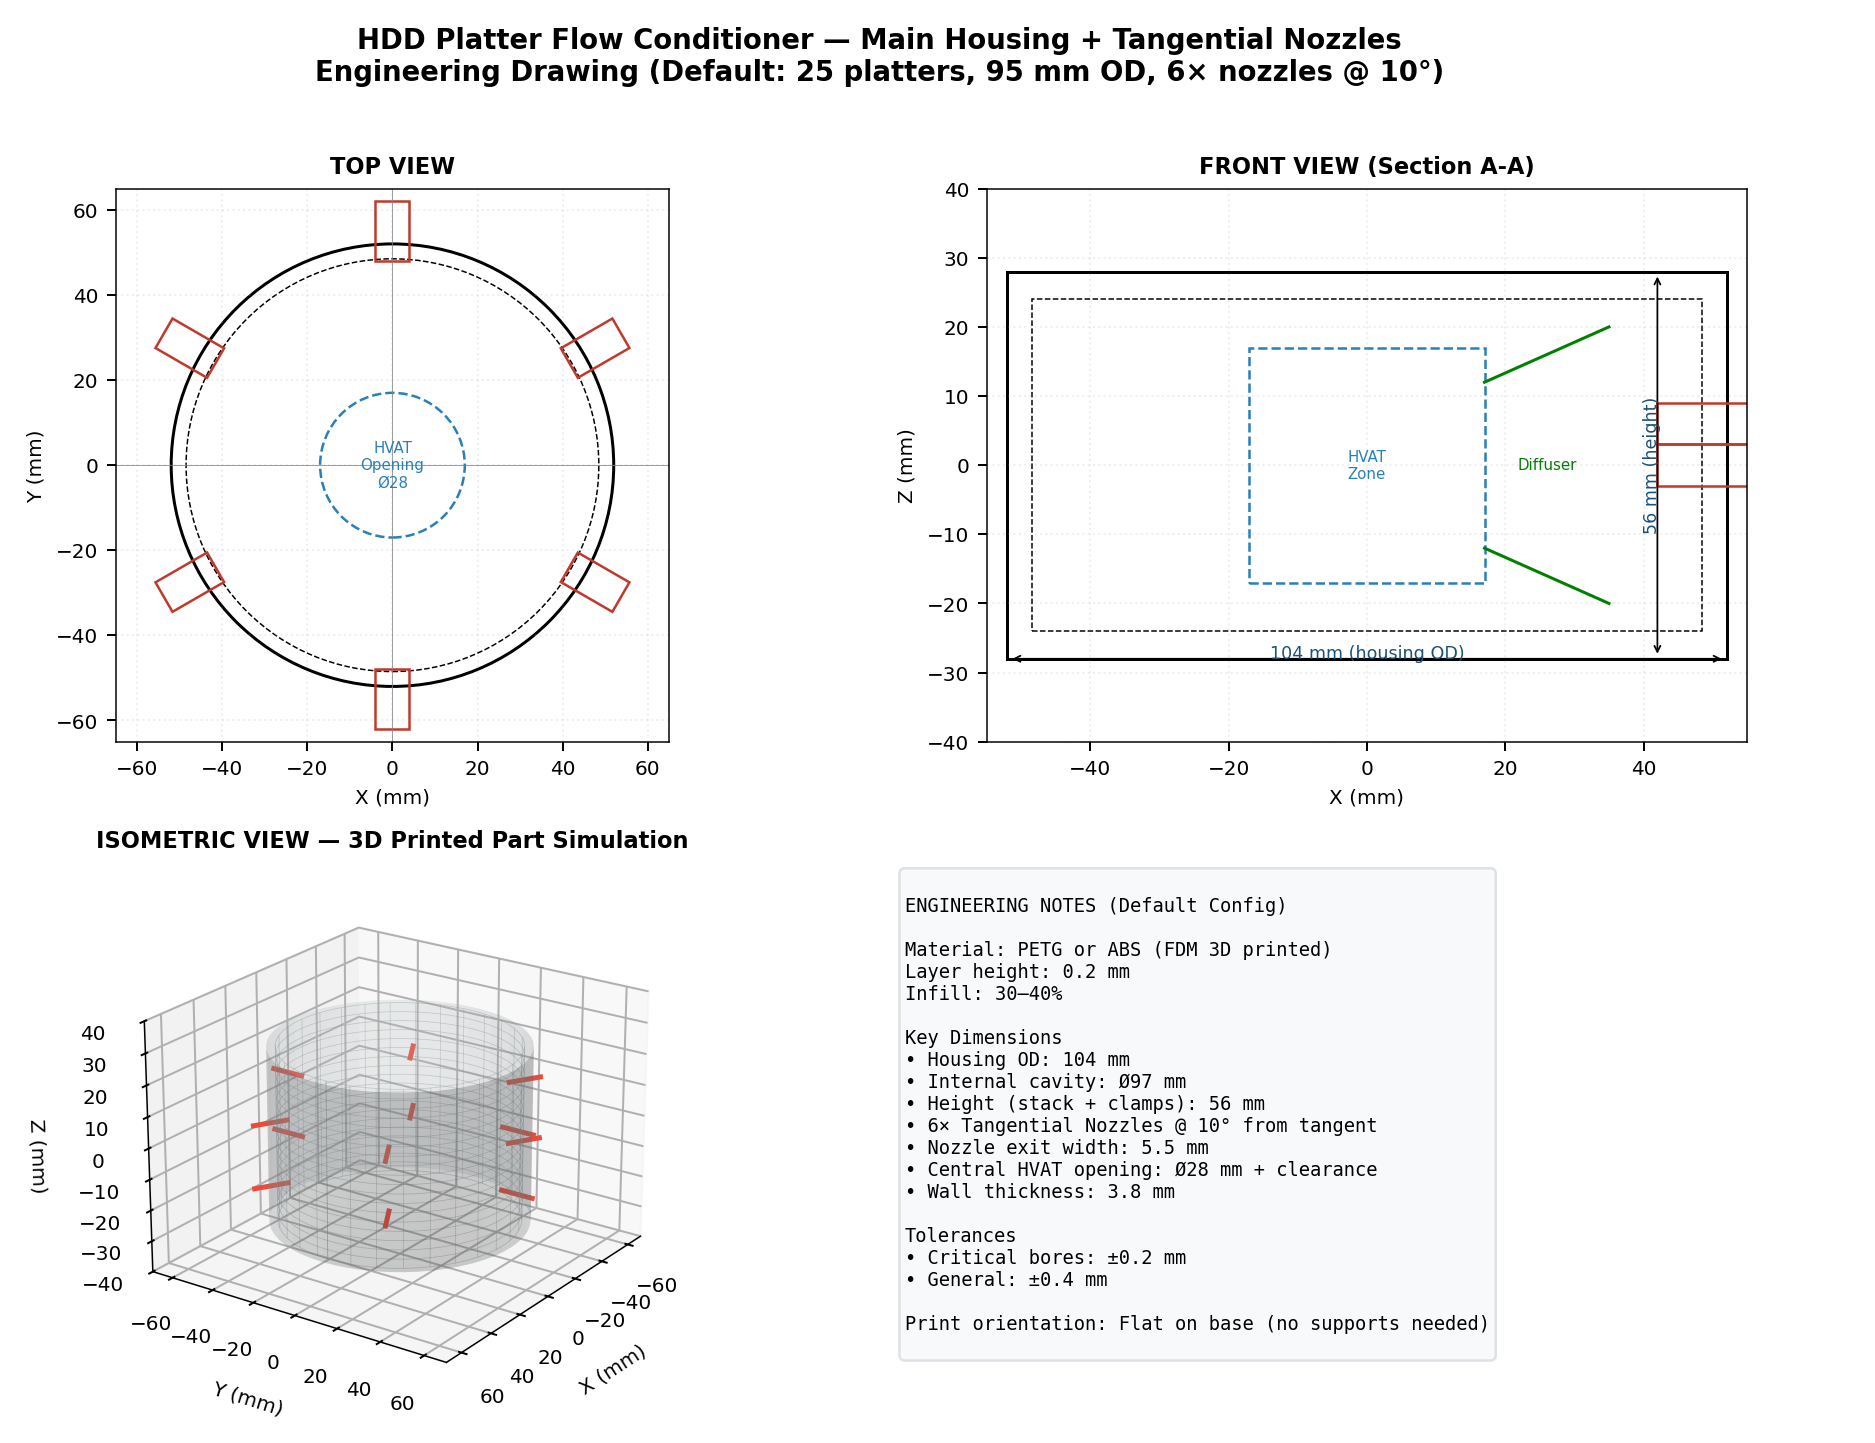
\includegraphics[width=\textwidth]{engineering_drawing_housing}
\caption{Main housing engineering drawing — Top and Front orthographic views with isometric simulation of the printed part.}
\label{fig:housing}
\end{figure}

\subsection{Hybrid VAWT (HVAT) Rotor}
The central active flow straightener combines Savonius starting scoops with helical Darrius blades (Figure~\ref{fig:hvat}).

\begin{figure}[H]
\centering
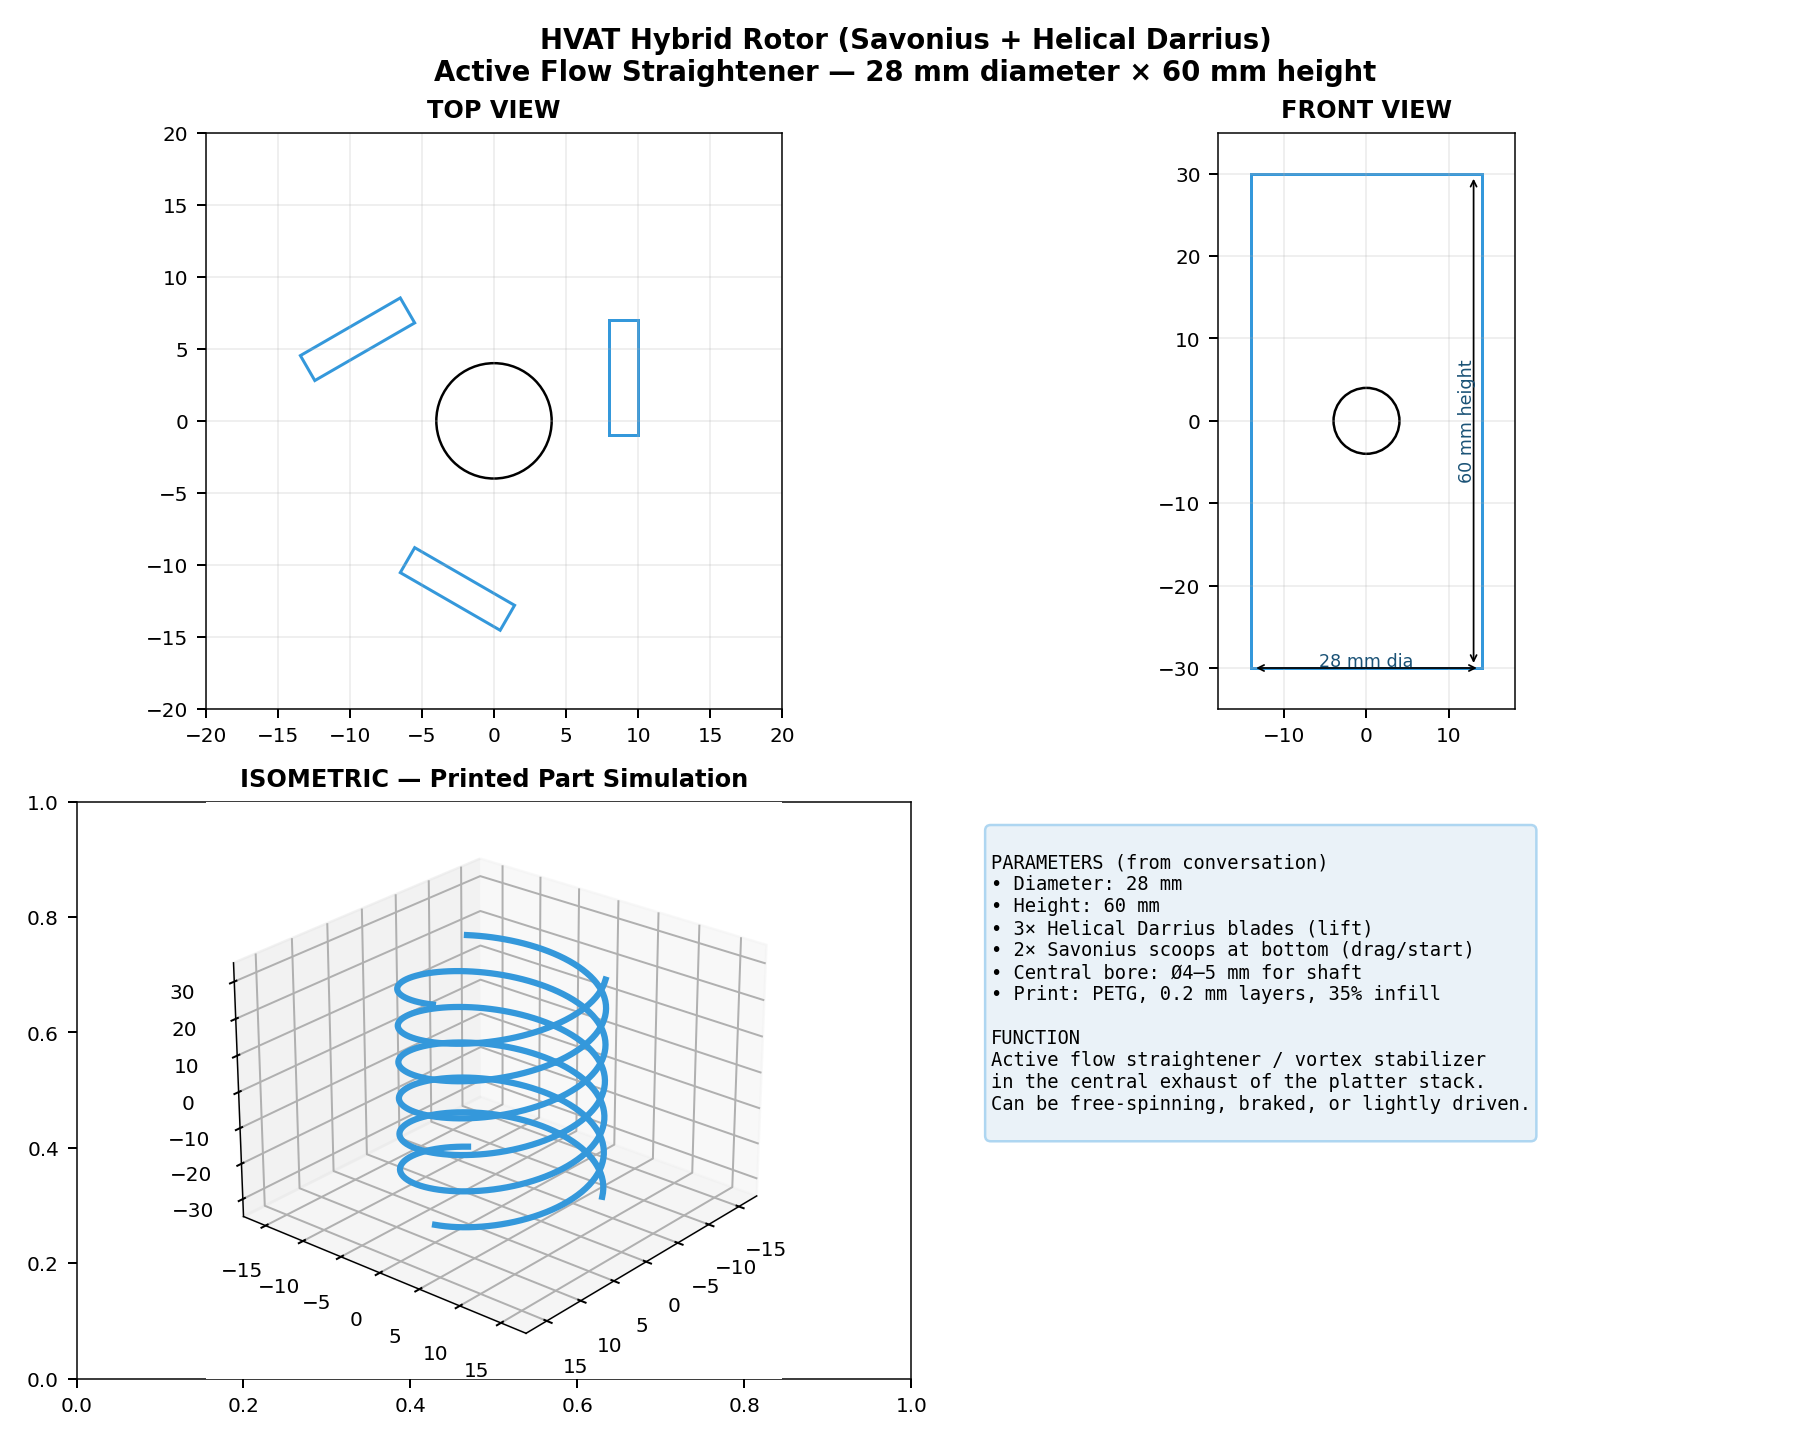
\includegraphics[width=0.95\textwidth]{engineering_drawing_hvat}
\caption{HVAT hybrid rotor — multi-view engineering drawing and 3D printed part simulation.}
\label{fig:hvat}
\end{figure}

\subsection{Cavitation Nozzle and Orifice Family}
The interchangeable orifices (6--12 mm) allow tuning of jet velocity and bubble dynamics without reprinting the entire nozzle (Figure~\ref{fig:nozzle}).

\begin{figure}[H]
\centering
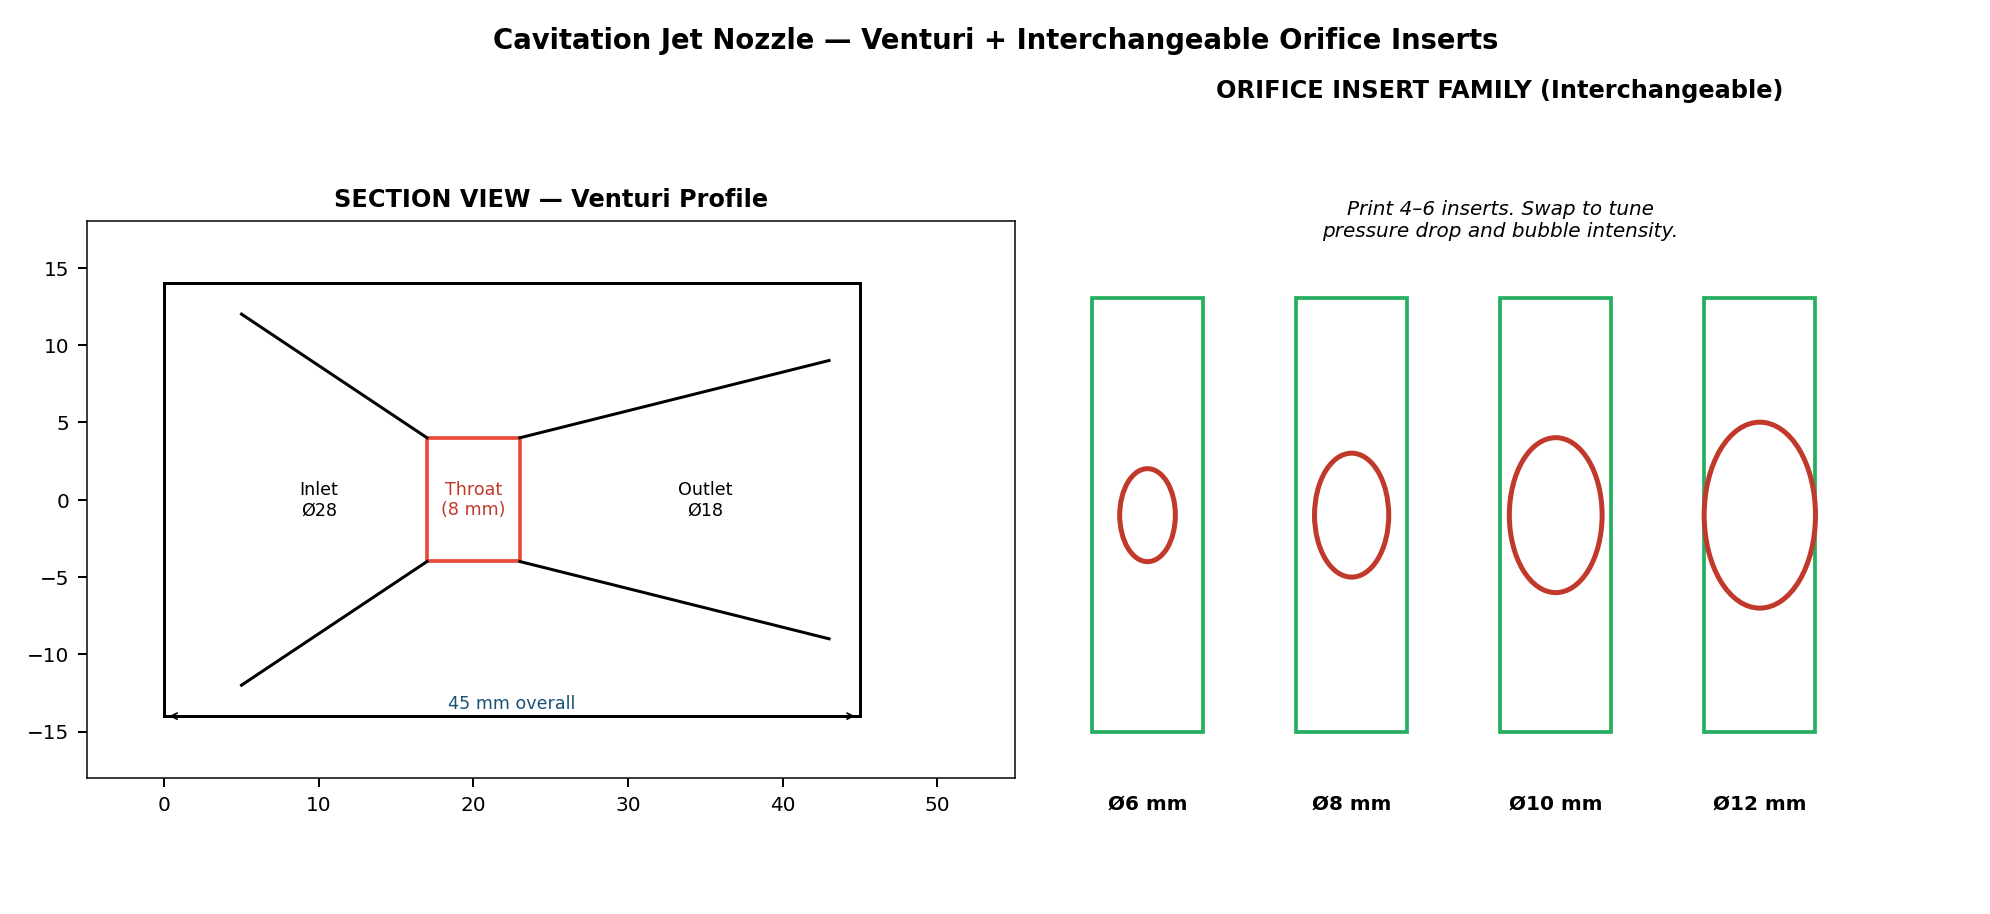
\includegraphics[width=\textwidth]{engineering_drawing_nozzle}
\caption{Cavitation jet nozzle — Venturi section view and complete set of orifice inserts.}
\label{fig:nozzle}
\end{figure}

\subsection{Assembly Tooling and Small Parts}
Critical small parts (Figure~\ref{fig:small}) ensure repeatable, high-precision builds.

\begin{figure}[H]
\centering
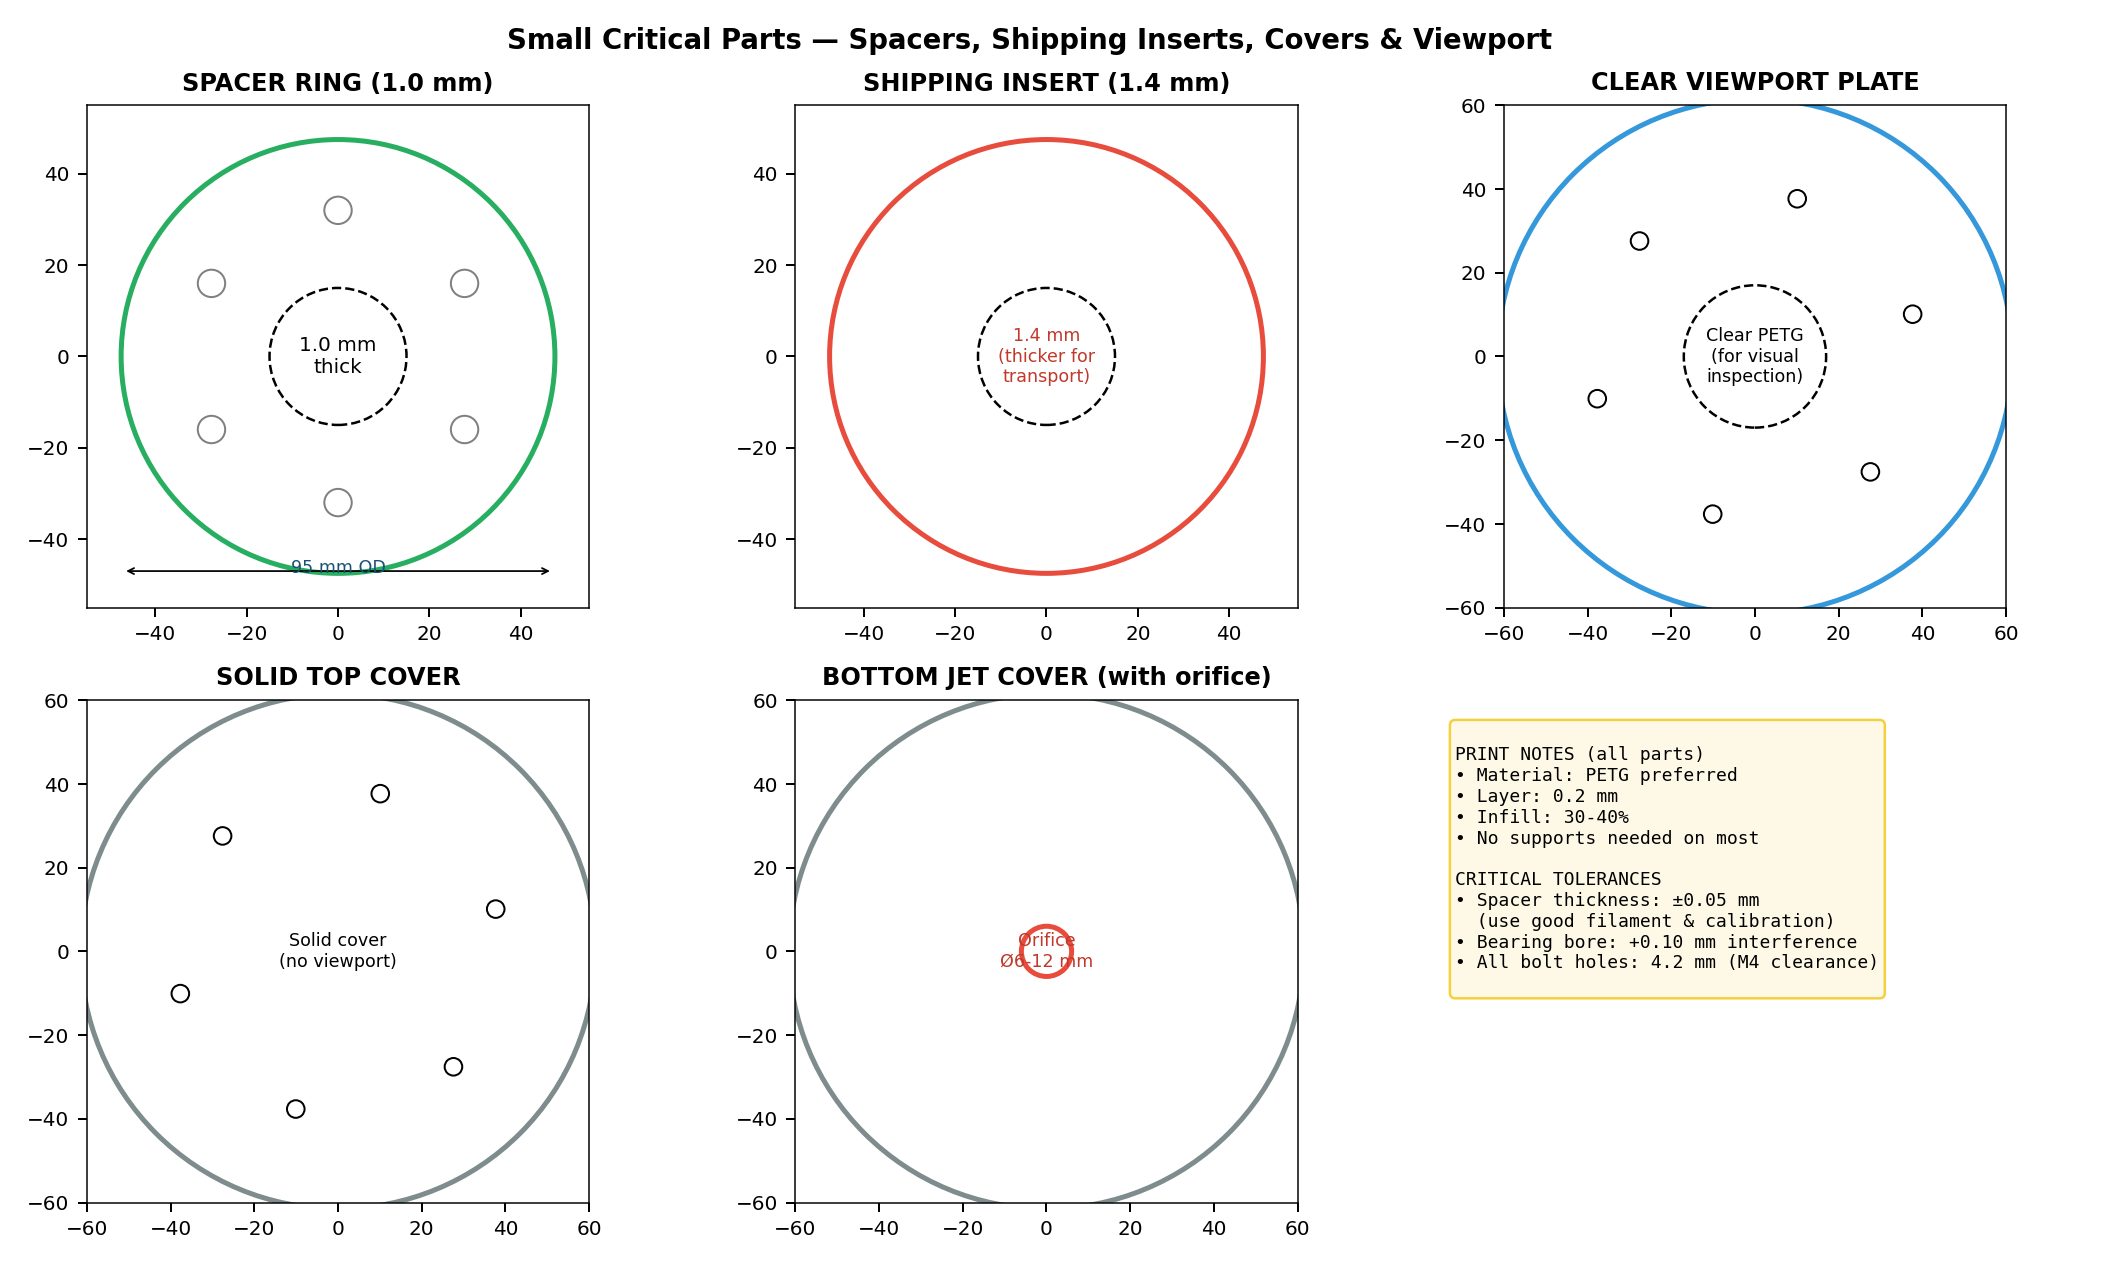
\includegraphics[width=\textwidth]{engineering_drawing_small_parts}
\caption{Spacer rings, shipping inserts, clear viewport, and solid covers — essential for gap control and safe transport.}
\label{fig:small}
\end{figure}

\clearpage

\subsection{Exploded and Assembled Views}
Figures~\ref{fig:exploded} and \ref{fig:assembled} provide overall understanding of how the device goes together.

\begin{figure}[H]
\centering
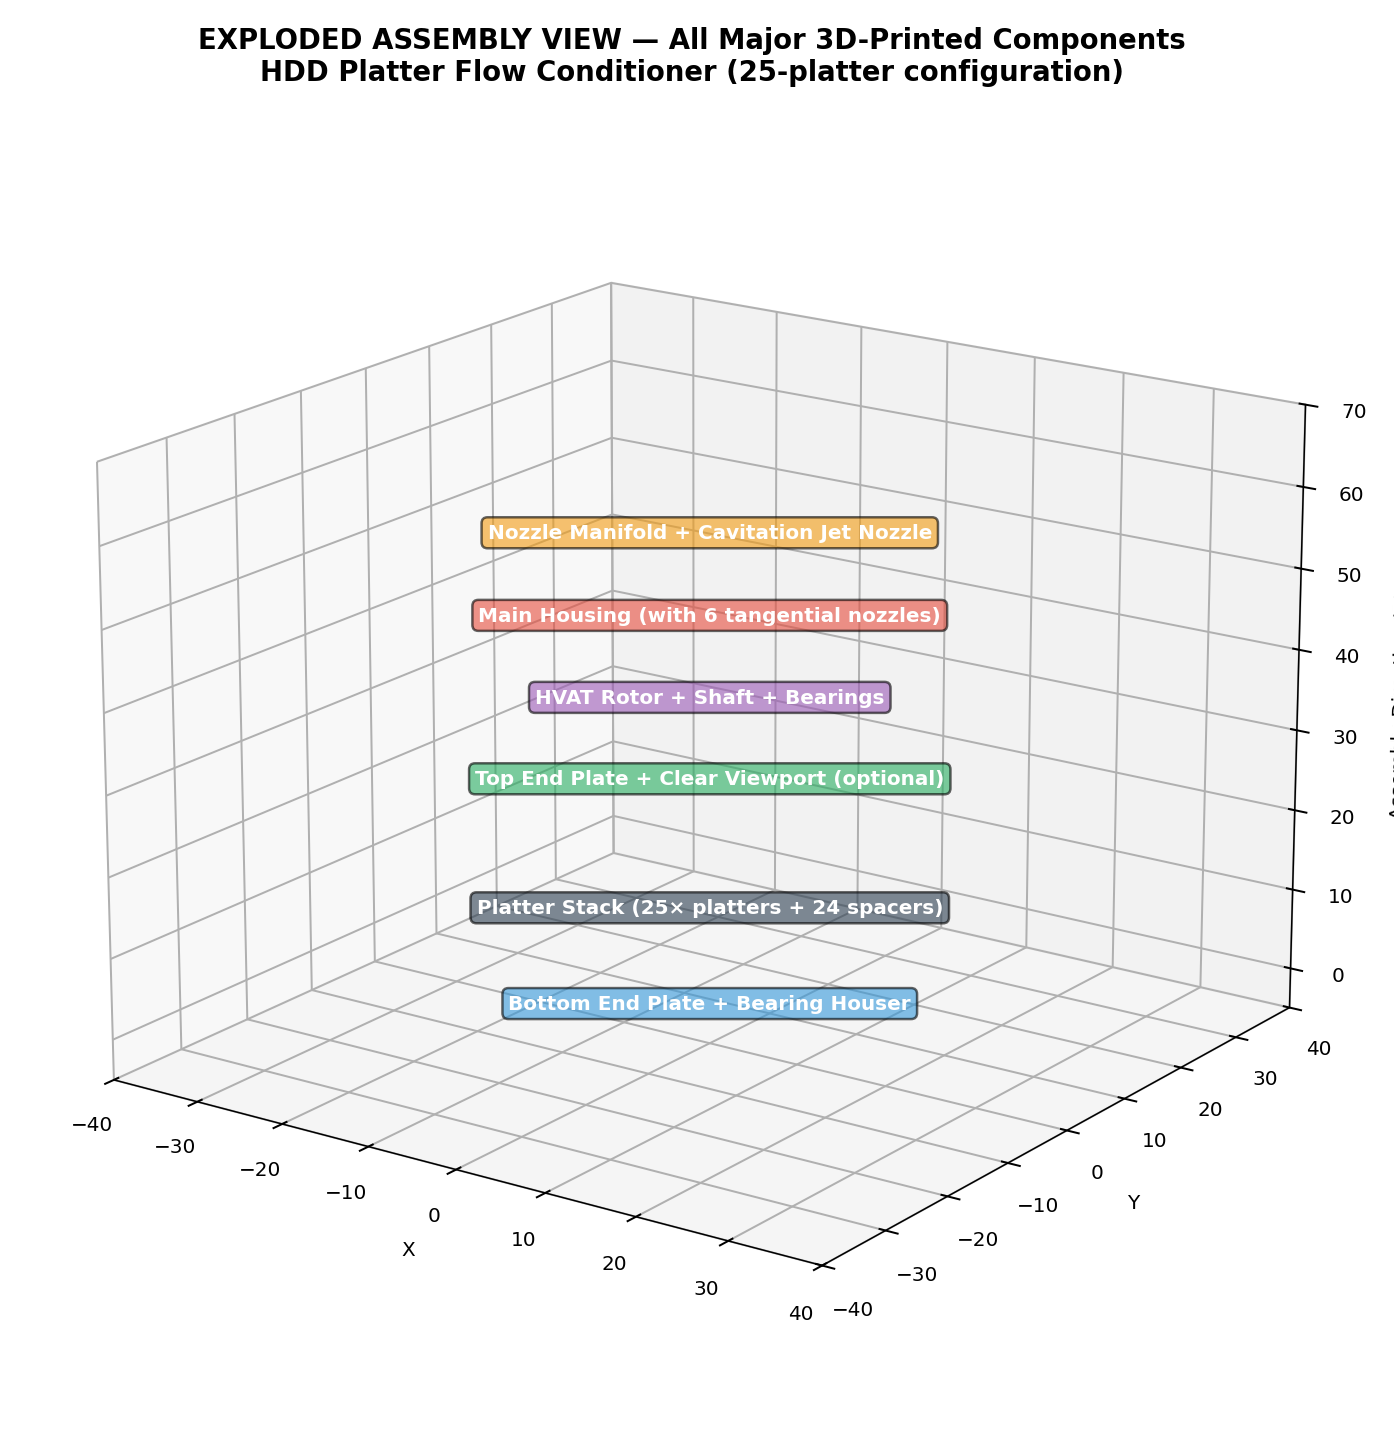
\includegraphics[width=0.9\textwidth]{exploded_assembly}
\caption{Exploded assembly view showing the logical stacking and mounting order of all major components.}
\label{fig:exploded}
\end{figure}

\begin{figure}[H]
\centering
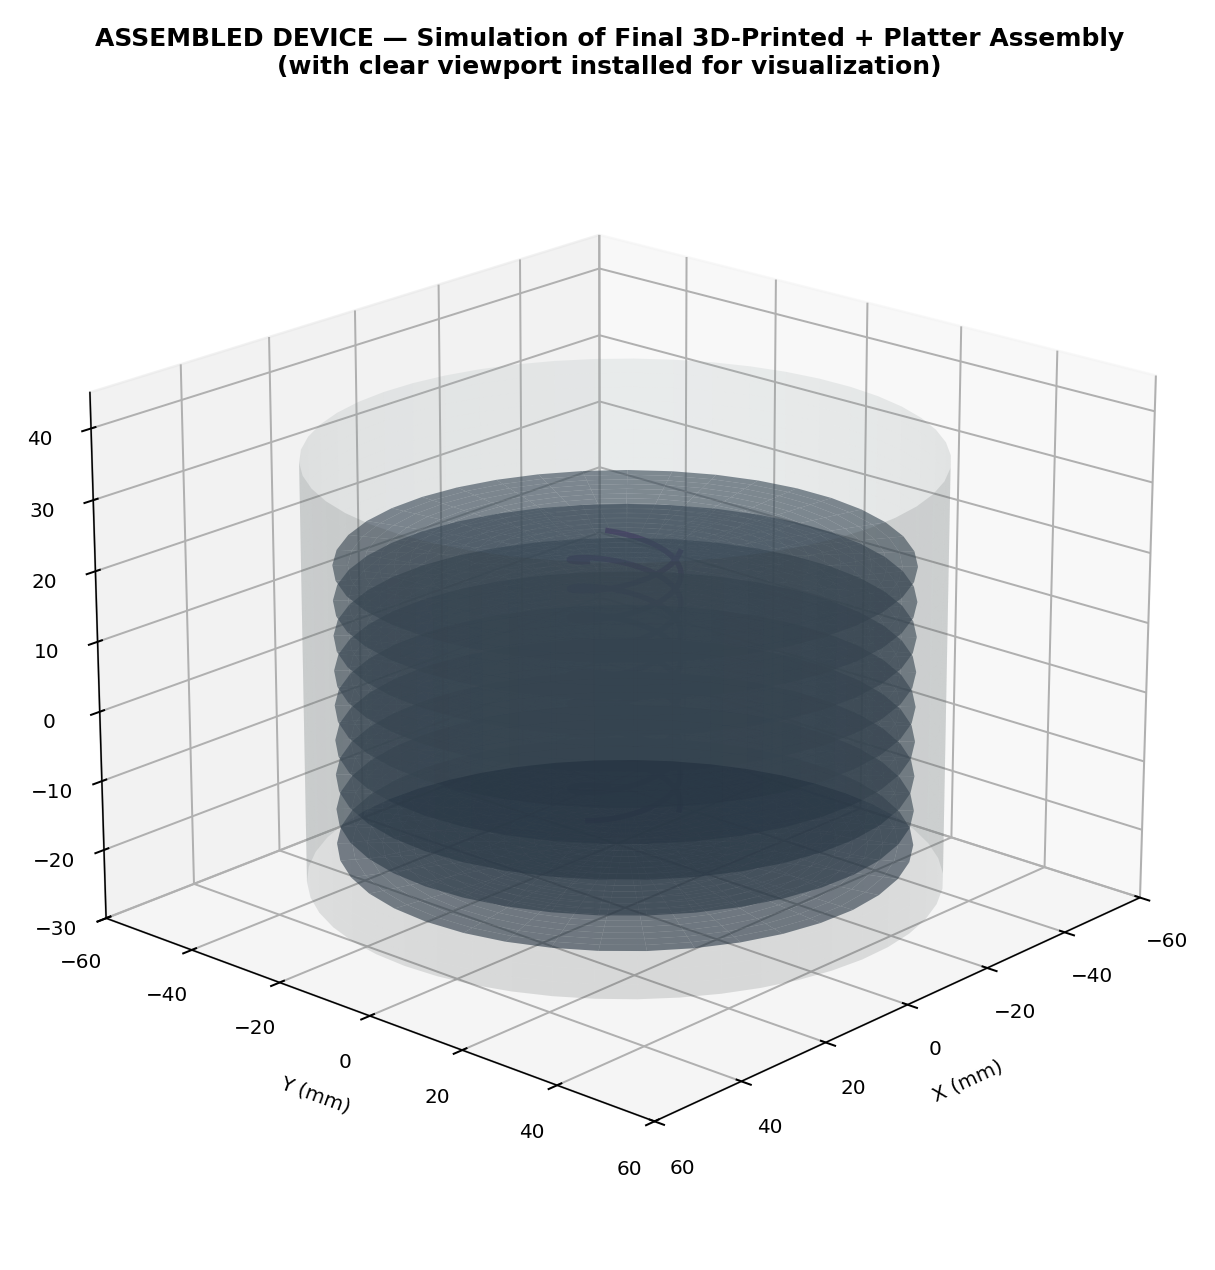
\includegraphics[width=0.85\textwidth]{assembled_device_simulation}
\caption{3D simulation of the fully assembled device with platter stack and HVAT rotor visible.}
\label{fig:assembled}
\end{figure}

\subsection{2D Fabrication Profiles (DXF)}
For laser cutting, CNC, or reference drilling, DXF profiles with proper layers (CUT, DRILL, ANNOTATE) are provided for the most fabrication-critical flat parts.

% Note: DXF files are provided separately in dxf_exports/ for laser/CNC use.
% They are not images and cannot be directly included here.

Full design rationale, detailed fluid dynamics explanation of how the device is expected to function, practical setup/tuning/testing protocols, and discussion of its unique value to Bob Greenyer / MFMP-style research are contained in the accompanying Sphinx documentation.

\clearpage

\subsection{Higher-Fidelity 3D Cutaway Views}
To aid understanding of internal geometry and flow paths, advanced 3D sectional visualizations have been generated programmatically.

\begin{figure}[H]
\centering
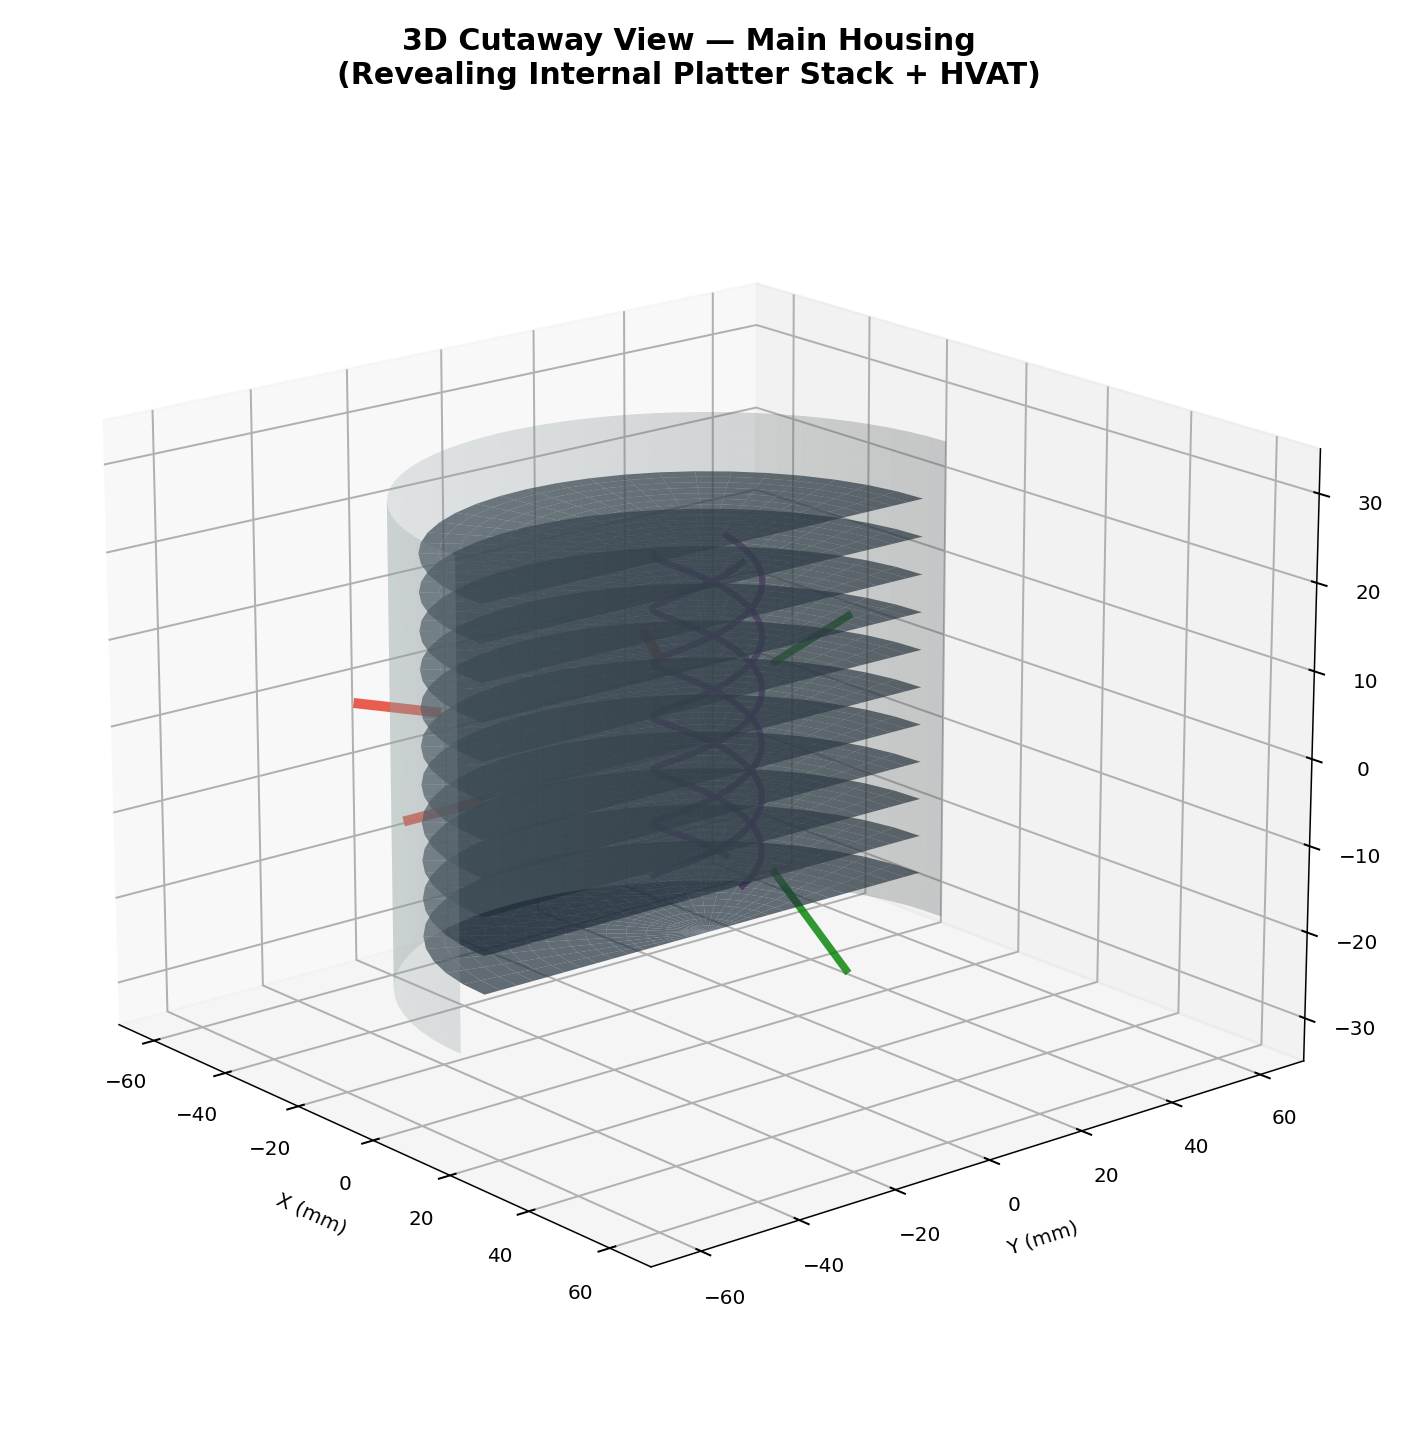
\includegraphics[width=\textwidth]{housing_cutaway_3d}
\caption{3D cutaway of the main housing revealing the internal platter stack and HVAT rotor.}
\end{figure}

\begin{figure}[H]
\centering
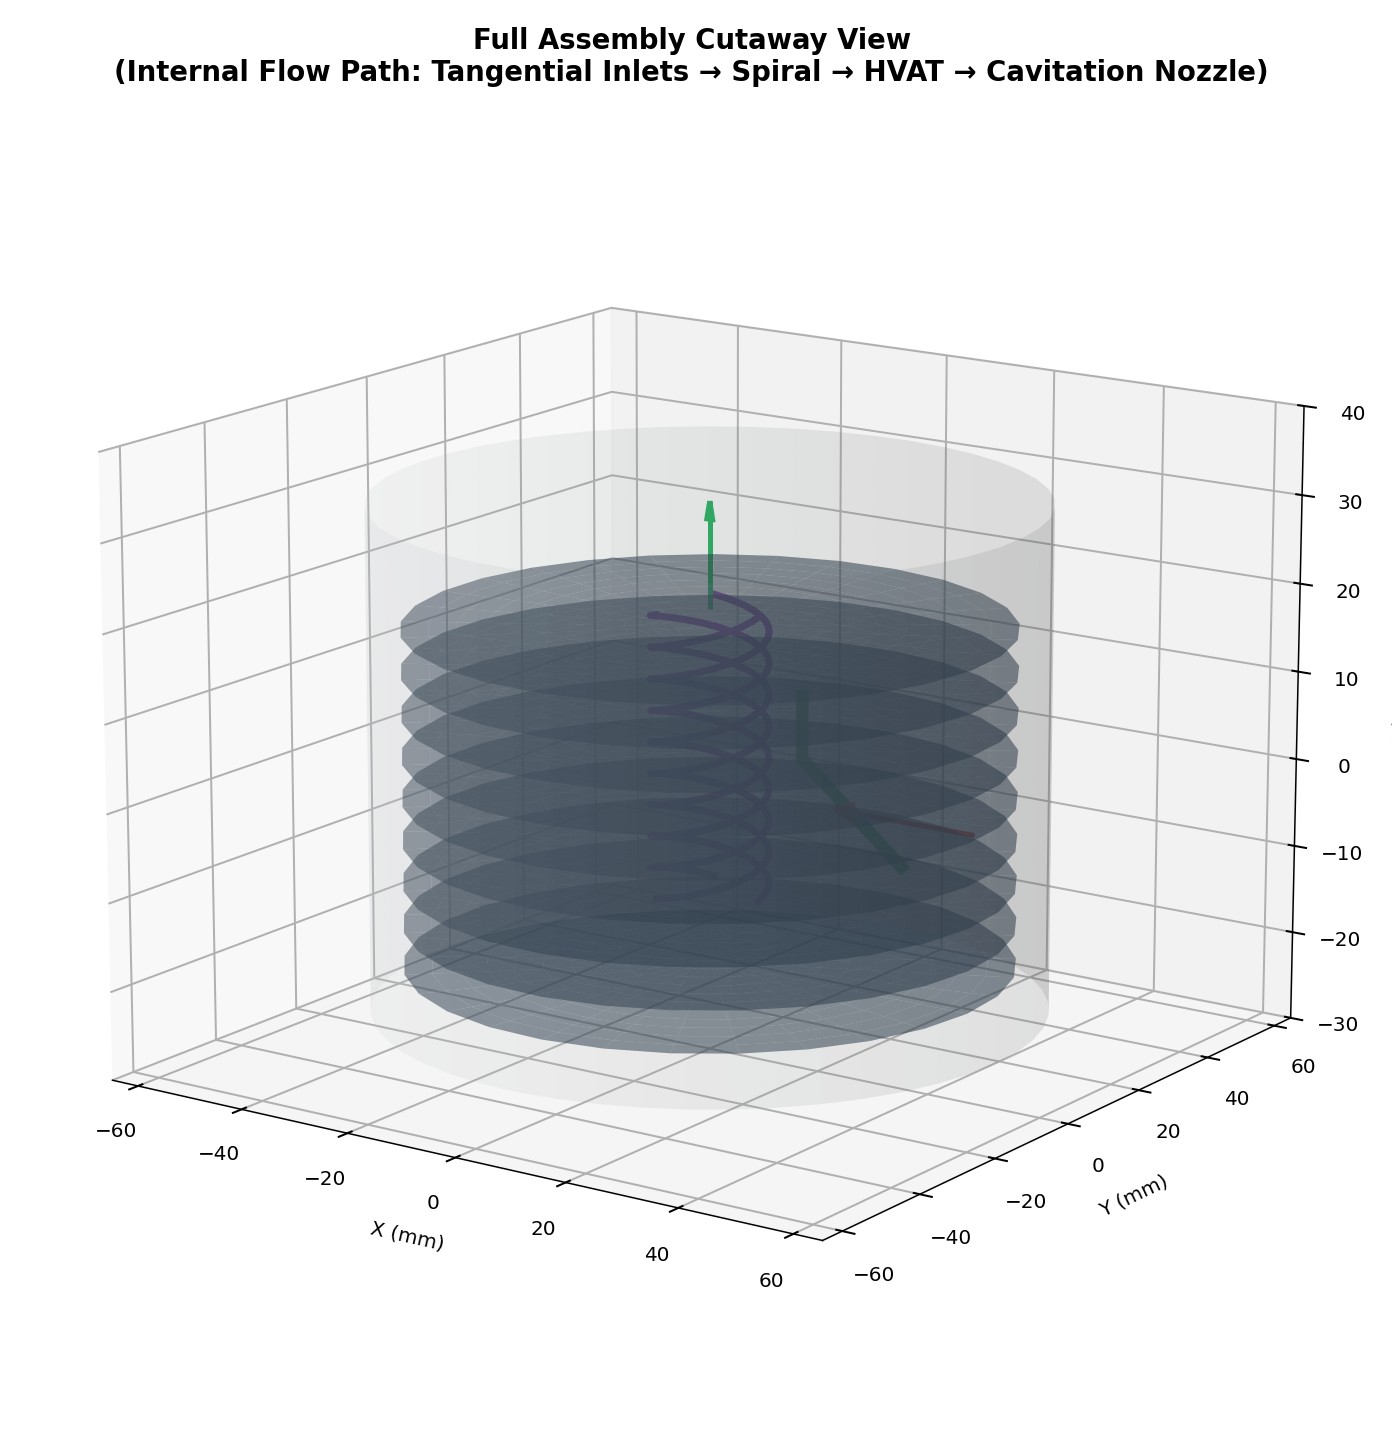
\includegraphics[width=\textwidth]{full_assembly_cutaway_3d}
\caption{Full assembly cutaway illustrating the complete internal flow path from tangential inlets through the spiral channels, HVAT, and into the cavitation nozzle.}
\end{figure}

\newpage
\bibliographystyle{plain}
\bibliography{references}

\end{document}
